%%%%%%%%%%%%%%%%%%%%%%%%%%%%%%%%%%%%%%%%%%%%%%%%%%%%%%%%%%%%%%%%%%%%%%%%%%%%%%%%
%              Capitulo 4: Arquitectura general del sistema                    %
%%%%%%%%%%%%%%%%%%%%%%%%%%%%%%%%%%%%%%%%%%%%%%%%%%%%%%%%%%%%%%%%%%%%%%%%%%%%%%%%

\chapter{Arquitectura general del sistema}

El sistema está estructurado en una serie de módulos lógicos que representan una
tarea de alto nivel. Un módulo lógico se compone a su vez de diversos módulos
funcionales o procesos, los cuáles llevan a cabo una tarea concreta y se comunican con
otros módulos funcionales del mismo módulo lógico para llevar a cabo dicha tarea de alto
nivel.

La tarea que un módulo funcional lleva a cabo puede realizarse de forma automática o
puede llegar a requerir de la interacción con el usuario para poder ser completada.
Cabe destacar además que, en determinados casos, los módulos funcionales de un módulo
lógico pueden comunicarse con los módulos funcionales de otros módulos lógicos, lo cuál se
describirá más detenidamente más adelante.

Por lo pronto, los módulos lógicos principales que se han considerado a la hora de definir
la arquitectura son los siguientes:

\begin{itemize}[label=\textbullet]
    \item Un módulo de interacción con el usuario (\textit{User interaction}).
    \item Un módulo de planificación (\textit{Planning}).
    \item Un módulo de monitorización y ejecución del plan (\textit{Plan Execution \& Monitoring}).
\end{itemize}

En la figura \ref{fig:system_arch} pueden verse los distintos módulos lógicos y funcionales que
componen el sistema, además de cómo están organizados, cómo se comunican y qué información se
envían entre ellos.

\begin{figure}[H]
    \centering
    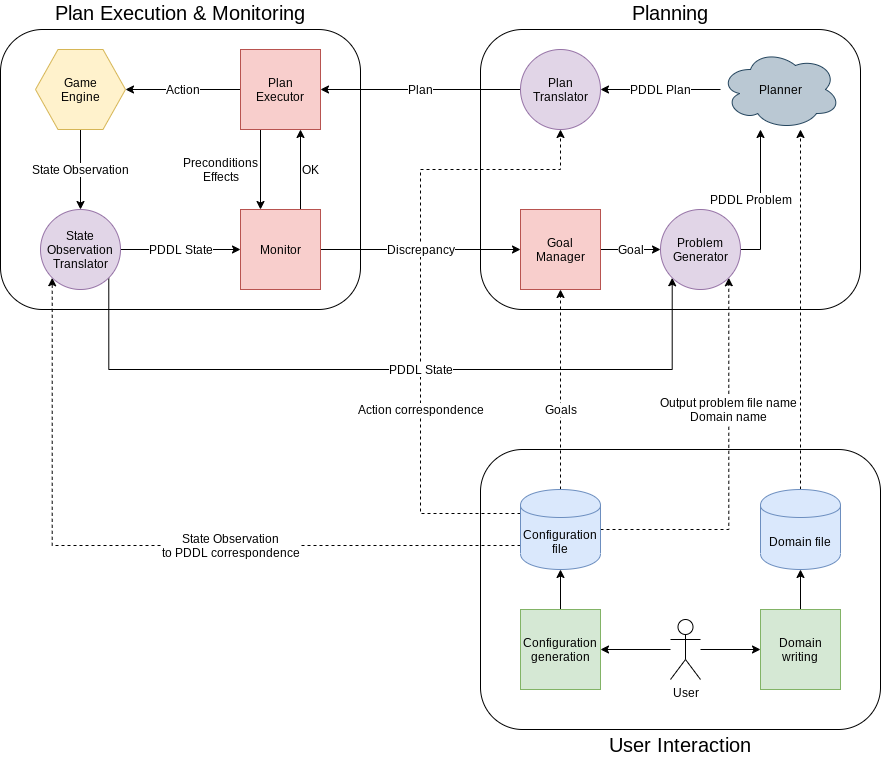
\includegraphics[scale=0.4]{img/CH04/system_arch.png}
    \caption{Esquema de la arquitectura general del sistema.}
    \label{fig:system_arch}
\end{figure}

Las distintas figuras, colores y flechas que se han utilizado a la hora de construir el
esquema representan lo siguiente:

\begin{itemize}[label=\textbullet]
    \item Los cilindros azules representan ficheros que se utilizan en el sistema.
    \item Los círculos de color morado representan módulos funcionales que llevan a cabo
    tareas de traducción.
    \item Los cuadrados representan módulos funcionales que realizan distintos tipos de
    tareas. Según el color que tengan, las tareas llevadas a cabo tendrán un mayor o menor
    grado de automatización:
    \begin{itemize}[label=\textendash]
        \item El color rojo se utiliza en tareas que se llevan a cabo automáticamente.
        \item El color verde se utiliza en tareas que requieren de la interacción del usuario
        en un mayor o menor grado para poder ser completadas.
    \end{itemize}
    \item El hexágono amarillo representa el entorno de juego.
    \item La nube de color gris representa el planificador, el cuál es un servicio en la
    nube.
    \item Las flechas normales representan información que se envían distintos módulos
    funcionales entre ellos.
    \item Las flechas discontinuas representan información proveniente de los archivos.
\end{itemize}

%%%%%%%%%%%%%%%%%%%%%%%%%%%%%%%%%%%%%%%%%%%%%%%%%%%%%%%%%%%%%%%%%%%%%%%%%%%%%%%%
%              Sección 4.1: Descripción general de la arquitectura             %
%%%%%%%%%%%%%%%%%%%%%%%%%%%%%%%%%%%%%%%%%%%%%%%%%%%%%%%%%%%%%%%%%%%%%%%%%%%%%%%%

\section{Descripción general de los módulos lógicos}

Vista la arquitectura 